\section{Spacecraft Configuration}
\label{sec:spacecraft_config}
The Spacecraft Options file (extension: {\tt .emtg\_spacecraftopt}) specifies
the capabilities of the spacecraft used in obtaining a solution with \ac{EMTG}, including information regarding the propulsion and power systems. These options files are considerably more detailed than the Launch Vehicle Options files.

The spacecraft options file is organized into various sections of data labeled ``Blocks''. A spacecraft is defined in the file within the {\tt \#BeginSpacecraftBlock} section of data. This section contains all required information in defining a spacecraft, including globally relevant data as well as additional blocks which define the power system and propulsion system information. The spacecraft options file also allows for multiple ``stages'', where each stage allows a user to change the spacecraft hardware characteristics. This information is contained within the {\tt \#BeginStageBlock} section of data. Each stage block contains information which is independent of data in other stage blocks. These blocks contain some unblocked data (such as masses and flags for constraints), a power system block identified by {\tt \#BeginStagePowerLibraryBlock}, and a propulsion system block identified by {\tt \#BeginStagePropulsionLibraryBlock}. The power and propulsion blocks are closed via a line {\tt \#EndHardwareBlock}, the stage blocks are ended via {\tt \#EndStageBlock}, and the spacecraft block is ended with {\tt \#EndSpacecraftBlock}. A {\tt .emtg\_spacecraftopt} file is thus organized as shown in Figure \ref{fig:config_spacecraftopt_organization}.

\begin{figure}[H]
    \center
    \begin{tabular}{l}
    {\tt \#BeginSpacecraftBlock} \\
    \hspace{2em} {Global Spacecraft Data} \vspace{0.05in} \\
    \hspace{2em} {\tt \#BeginStageBlock} \\
    \hspace{4em} {General Information for Stage 1} \vspace{0.05in} \\
    \hspace{4em} {\tt \#BeginStagePowerLibraryBlock} \\
    \hspace{6em} {Power System Definition} \\
    \hspace{4em} {\tt \#EndHardwareBlock} \vspace{0.05in} \\
    \hspace{4em} {\tt \#BeginStagePropulsionLibraryBlock} \\
    \hspace{6em} {Propulsion System Definition} \\
    \hspace{4em} {\tt \#EndHardwareBlock} \vspace{0.05in} \\
    \hspace{2em} {\tt \#EndStageBlock} \vspace{0.05in} \\
    {\tt \#EndSpacecraftBlock}
    \end{tabular}
\caption{Example Structure Of {\tt .emtg\_spacecraftopt} Files}
\label{fig:config_spacecraftopt_organization}
\end{figure}

\subsection{Spacecraft Block}
The spacecraft block section contains the globally relevant data for defining a spacecraft in \ac{EMTG} as well as at least one stage block containing power and propulsion system definitions. The global data contained in the spacecraft block sets the name of the spacecraft, flags for enabling or disabling maximum values on propellant and dry mass, and minimum/maximum values for constraints that are enabled. The lines and expected data types are shown in Table \ref{tab:spacecraftblock_globals} followed by additional details per item.

\begin{table}[H]
    \centering
    % \begin{tabular}{l|l|l}
    \begin{tabular}{llll}
    \hline
    \textbf{Line} & \textbf{Variable} & \textbf{Line Name} & \textbf{Data Type} \\
    \hline
    \textbf{1} & 1 & Name & String \\
    % \hline
    \textbf{2} & 1 & EnableGlobalElectricPropellantTankConstraint & Boolean Integer \\
    % \hline
    \textbf{3} & 1 & EnableGlobalChemicalPropellantTankConstraint & Boolean Integer \\
    % \hline
    \textbf{4} & 1 & EnableGlobalDryMassConstraint & Boolean Integer \\
    % \hline
    \textbf{5} & 1 & GlobalElectricPropellantTankCapacity & Real (kg) \\
    % \hline
    \textbf{6} & 1 & GlobalFuelTankCapacity & Real (kg) \\
    % \hline
    \textbf{7} & 1 & GlobalOxidizerTankCapacity & Real (kg) \\
    % \hline
    \textbf{8} & 1 & GlobalDryMassBounds & Real (kg) \\ & & & ($\ge$ 0, $\le$ GlobalDryMassBounds[1]) \\
    \textbf{8} & 2 & GlobalDryMassBounds & Real (kg) \\ & & & ($\ge$ GlobalDryMassBounds[0]) \\
    \end{tabular}
    \caption{Spacecraft Block Global Data}
    \label{tab:spacecraftblock_globals}
\end{table}


\listitem{Name}{The name of the spacecraft.}
\listitem{EnableGlobalElectricPropellantTankConstraint}{A boolean integer enabling a global bound on the electric propellant tank maximum capacity.}
\listitem{EnableGlobalChemicalPropellantTankConstraint}{A boolean integer enabling a global bound on the chemical propellant tank maximum capacity.}
\listitem{EnableGlobalDryMassConstraint}{A boolean integer enabling lower and upper bounds on the global dry mass.}
\listitem{GlobalElectricPropellantTankCapacity}{Maximum electric propellant mass, in kilograms.}
\listitem{GlobalFuelTankCapacity}{Maximum chemical fuel mass, in kilograms.}
\listitem{GlobalOxidizerTankCapacity}{Maximum oxidizer mass, in kilograms.}
\listitem{GlobalDryMassBounds}{Lower and upper bounds on the global dry mass, provided as two space-delimited variables, where the first defines the lower bound and the second defines the upper bound. The bound values are only considered if the corresponding constraint is active.}

The spacecraft block example shown in Figure \ref{fig:config_spacecraftblock} demonstrates the usage of these mass constraints. While the chemical fuel tank capacity has a value of 1000 kg, the constraint is not active since the corresponding enable flag is set to ``0''. Conversely, the global dry mass constraint is active and thus the lower and upper bounds of 1000 kg and 1500 kg as set by the GlobalDryMassBounds line are active.


\begin{figure}[htb]
    \centering
    \begin{tabular}{|l|}
        \hline
        {\tt \#BeginSpacecraftBlock} \\
        {\tt name example\_spacecraft} \\
        {\tt EnableGlobalElectricPropellantTankConstraint 1} \\
        {\tt EnableGlobalChemicalPropellantTankConstraint 0} \\
        {\tt EnableGlobalDryMassConstraint 1} \\
        {\tt GlobalElectricPropellantTankCapacity 1000} \\
        {\tt GlobalFuelTankCapacity 1000} \\
        {\tt GlobalOxidizerTankCapacity 1000} \\
        {\tt GlobalDryMassBounds 1000 1500} \\
        \hline
    \end{tabular}
    \caption{Example Spacecraft Block Global Data}
    \label{fig:config_spacecraftblock}
\end{figure}


\subsection{Stage Block General Data}
\label{sec:stage_block_data}
After the Spacecraft Block data and still within the {\tt \#BeginSpacecraftBlock}, there are one or more Stage Block sections, bounded by {\tt \#BeginStageBlock} and {\tt \#EndStageBlock}. This section is similar to the Spacecraft Block and contains stage masses, boolean integers for enabling or disabling mass constraints, maximum masses for the fuel tanks of a stage if the associated constraint is applied, throttle logic and sharpness settings, and information regarding the power and propulsion systems. The lines and expected data types for the general stage information are shown in Table \ref{tab:spacecraft_stage_block_general} with additional details subsequently provided, and an example is provided in Figure \ref{fig:config_stageblock}. The power system is defined within a Stage Power Library Block, while the propulsion systems are defined within a Stage Propulsion Library Block contained within the Stage Block. This terminology is also detailed in Section 5.4 of the \ac{EMTG} Software Design Document.

\begin{table}[ht]
    \centering
    % \begin{tabular}{l|l|l}
    \begin{tabular}{lll}
    \hline
    \textbf{Line} & \textbf{Line Name} & \textbf{Data Type} \\
    \hline
    \textbf{1} & Name & String \\
    % \hline
    \textbf{2} & BaseDryMass & Real (kg) \\
    % \hline
    \textbf{3} & AdapterMass & Real (kg) \\
    % \hline
    \textbf{4} & EnableElectricPropellantTankConstraint & Boolean Integer \\
    % \hline
    \textbf{5} & EnableChemicalPropellantTankConstraint & Boolean Integer\\
    % \hline
    \textbf{6} & EnableDryMassConstraint & Boolean Integer \\
    % \hline
    \textbf{7} & ElectricPropellantTankCapacity & Real (kg) \\
    % \hline
    \textbf{8} & ChemicalFuelTankCapacity & Real (kg) \\
    % \hline
    \textbf{9} & ChemicalOxidizerTankCapacity & Real (kg) \\
    % \hline
    \textbf{10} & ThrottleLogic & Integer (1: min number of thrusters, \\ & & \hspace{3em}\hspace{5pt} 2: max number of thrusters) \\
    % \hline
    \textbf{11} & ThrottleSharpness & Real (> 0) \\
    % \hline
    \textbf{12} & PowerSystem & String (name of power system) \\
    % \hline
    \textbf{13} & ElectricPropulsionSystem & String (name of electric propulsion system) \\
    % \hline
    \textbf{14} & ChemicalPropulsionSystem & String (name of chemical propulsion system) \\
    % \hline
    \end{tabular}
    \caption{Stage Block Data}
    \label{tab:spacecraft_stage_block_general}
\end{table}

\listitem{Name}{The name of the stage.}
\listitem{BaseDryMass}{The dry mass of the propulsion system base, in kilograms.}
\listitem{AdapterMass}{Mass of the spacecraft-to-power-system adapter, in kilograms.}
\listitem{EnableElectricPropellantTankConstraint}{A boolean integer enabling a bound on the electric propellant tank maximum capacity.}
\listitem{EnableChemicalPropellantTankConstraint}{A boolean integer enabling a bound on the chemical propellant tank maximum capacity.}
\listitem{EnableDryMassConstraint}{A boolean integer option for bounding the final mass at the end of a stage to be greater than the required mass, which is a sum of dry mass and other system masses. Users do not set bounds for this constraint. Instead, if this constraint is active, then the final mass at the end of the stage must be greater than the required mass at the end of the stage. The required mass is the sum of the stage block dry mass, stage electric propulsion system mass, stage chemical propulsion system mass, stage power system mass, electric propellant mass margin, chemical fuel mass margin, and chemical oxidizer mass margin. The fractional margins are set in the {\tt .emtgopt} file as {\tt electric\_propellant\_margin} and {\tt chemical\_propellant\_margin} and may be set in the PyEMTG interface in the ``Spacecraft Options'' tab under the ``Margins'' header.}
\listitem{ElectricPropellantTankCapacity}{Maximum electric propellant mass, in kilograms.}
\listitem{ChemicalFuelTankCapacity}{Maximum chemical fuel mass, in kilograms.}
\listitem{ChemicalOxidizerTankCapacity}{Maximum oxidizer mass, in kilograms.}
\listitem{ThrottleLogic}{Integer (1 or 2) defining logic for selecting the number of thrusters. Users may choose between firing either the minimum ({\tt ThrottleLogic = 1}) or maximum ({\tt ThrottleLogic = 2}) number of thrusters possible for a given amount of available power. The {\tt MaxThrusters} option typically results in thrusters fired close to their minimum power, resulting in poor performance, while the {\tt MinThrusters} often results in thrusters being fired closer to their maximum power, resulting in better performance. While at first glance it may seem that the {\tt MinThrusters} option would consistently be best, the choice of throttle logic for a given problem can sometimes be unintuitive.}
\listitem{ThrottleSharpness}{Defines how quickly the thruster transitions between different settings. A larger value indicates a steeper curve and faster transition. The throttle sharpness model uses an approximation of the discontinuous Heaviside step function $\bar{H}_i$ via a logistic function, where {\it k} is the throttle sharpness, $P_a$ is the continuously defined power available to the Power Processing Unit (PPU), and $P_i$ defines a power level, where $P_i \in {P_1, P_2, ..., P_n}$. The function can then be defined as shown in equation \ref{eq:heaviside_throttle_sharpness} and is shown in Figure \ref{fig:heaviside_throttle_sharpness}, where $x = (P_a - P_i)$. \\
\begin{equation}
    \bar{H}_i = \frac{1}{1 + e^{-k (P_a - P_i)}}
    \label{eq:heaviside_throttle_sharpness}
\end{equation}
\begin{figure}[H]
    \center
    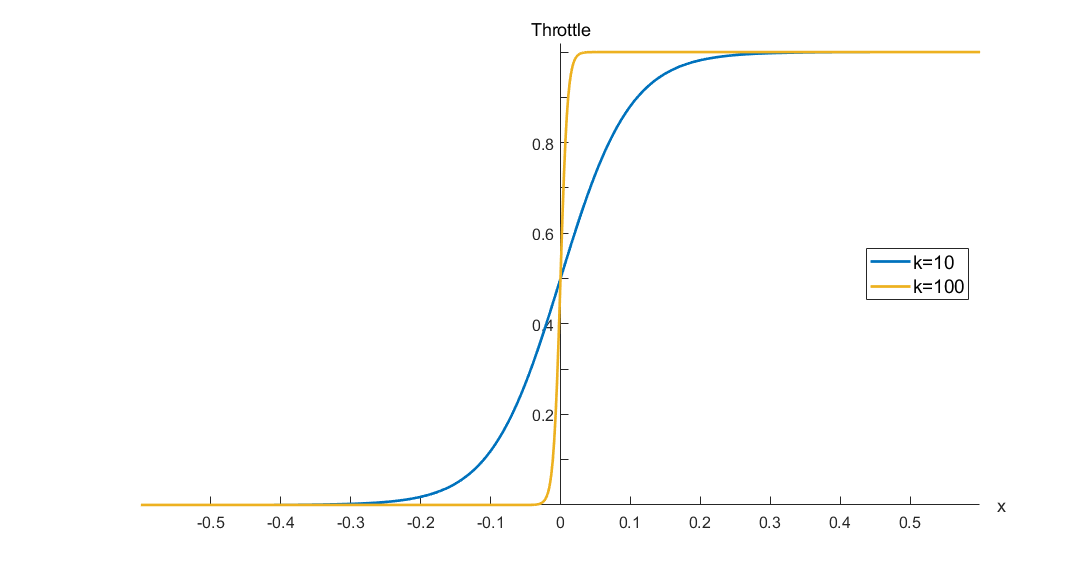
\includegraphics[width=0.95\linewidth]{../../shared_latex_inputs/images/throttle_sharpness_curve.png}
    \caption{Throttle Sharpness}
    \label{fig:heaviside_throttle_sharpness}
\end{figure}
These throttle options are available to allow for more precise tuning of throttle table calculations. The Electric Propulsion System in particular allows for 1D and 2D smooth-stepped electric thruster models which operate using a user-supplied set of discrete throttle points (provided in the {\tt .ThrottleTable} file). Since \ac{EMTG} is a gradient based optimization tool, the thrust and $I_{sp}$ provided in the throttle table must be first-differentiable with respect to input power. The logistic function approximation of the Heaviside function solves this differentiability problem. More precise mathematical detail of the usage of these throttle options including detailed information on the implementation of 1D throttling, 2D throttling, and multi-thruster switching is provided in section \ref{sec:electric_propulsion_system}. For further detail, see Section 5.6.2 (Electric Propulsion System Model) of the \ac{EMTG} Software Design Document.}
\listitem{PowerSystem}{Name of the power system for the stage, defined in the Power Library Block.}
\listitem{ElectricPropulsionSystem}{Name of the electric propulsion system for the stage, defined in the Propulsion Library Block.}
\listitem{ChemicalPropulsionSystem}{Name of the chemical propulsion system for the stage, defined in the Propulsion Library Block.}


\begin{figure}[H]
    \centering
    \begin{tabular}{|l|}
        \hline
        {\tt \#BeginStageBlock} \\
        {\tt name Example\_Stage} \\
        {\tt BaseDryMass 0} \\
        {\tt AdapterMass 0} \\
        {\tt EnableElectricPropellantTankConstraint 0} \\
        {\tt EnableChemicalPropellantTankConstraint 0} \\
        {\tt EnableDryMassConstraint 0} \\
        {\tt ElectricPropellantTankCapacity 1000.0} \\
        {\tt ChemicalFuelTankCapacity 1000.0} \\
        {\tt ChemicalOxidizerTankCapacity 1000.0} \\
        {\tt ThrottleLogic 1} \\
        {\tt ThrottleSharpness 100} \\
        {\tt PowerSystem LowSIRIS\_Power} \\
        {\tt ElectricPropulsionSystem LowSIRIS\_ElectricProp} \\
        {\tt ChemicalPropulsionSystem LowSIRIS\_ChemicalProp} \\
        \hline
    \end{tabular}
    \caption{Example Spacecraft Stage Block Data}
    \label{fig:config_stageblock}
\end{figure}



\subsection{Power System}
\label{sec:power_system}
The power system is defined as an option contained in a Power Library Block. This is either defined with a {\tt .emtg\_powersystemsopt} file when setting ``Spacecraft model type'' to ``0: Assemble from libraries'' or within the Stage Block when using ``1: Read .emtg\_spacecraftoptions file''. In each case, the format is the same as detailed in this section and demonstrated in Figure \ref{fig:config_powerlibrary_block}. 

The power systems block allows for defining multiple power system options that can be easily interchanged, similar to the launch vehicle options file. This block is opened with {\tt \#BeginStagePowerLibraryBlock} and closed with {\tt \#EndHardwareBlock}. The information set here is that which would be set on the PyEMTG Spacecraft Options page in the ``Power options'' section if ``Spacecraft model type'' were set to ``2: Assemble from missionoptions object''.

In the Power Library Block, power systems are specified by a name followed by a series of comma- or space-delimited numbers on a single line. A stage can have multiple power systems specified, but only that specified in the general data in the Stage Block as the {\tt PowerSystem} will be used. Table \ref{tab:spacecraft_stage_powerlib_block} specifies the parameters and data types for each Power System, with additional details for each option subsequently provided.

\begin{table}[ht]
    \centering
    % \begin{tabular}{l|l|l}
    \begin{tabular}{lll}
    \hline
    \textbf{Index} & \textbf{Variable Name} & \textbf{Data Type} \\
    \hline
    \textbf{1} & Name & String \\
    % \hline
    \textbf{2} & Spacecraft\_Power\_Supply\_Type & Integer (0: Constant, 1: Solar) \\
    % \hline
    \textbf{3} & Spacecraft\_Power\_Supply\_Curve\_Type & Integer (0: Sauer, 1: Polynomial) \\
    % \hline
    \textbf{4} & Spacecraft\_Bus\_Power\_Type & Integer (0: Quadratic, \\ & & \hspace{3em}\hspace{5pt} 1: Conditional) \\
    % \hline
    \textbf{5} & P0 & Real (kW) \\
    % \hline
    \textbf{6} & mass\_per\_kW & Real (kg) \\
    % \hline
    \textbf{7} & decay\_rate & Real (1/years) \\
    % \hline
    \textbf{8-14} & gamma[0:6] & Real \\
    % \hline
    \textbf{15-17} & BusPower[0:2] & Real \\
    % \hline
    \end{tabular}
    \caption{Power System Variables}
    \label{tab:spacecraft_stage_powerlib_block}
\end{table}


Items 2, 3, and 5-14 specify the power produced for the propulsion system, while items 4 and 15-17 specify the spacecraft power use for purposes other than electric propulsion (i.e., a non-zero bus power means that there is some amount of power produced by the spacecraft that cannot be used by the electric propulsion system). Figure \ref{fig:config_powerlibrary_block} provides an example power library block. In practice, early designs frequently make use of simple power models (e.g., the {\tt LowSIRIS\_Power} example in Figure \ref{fig:config_powerlibrary_block}) and move to more accurately modeled systems as the trajectory design process proceeds. Definitions of these variables follows. In some of the calculations defined by these variables, the distance of the spacecraft from the Sun, $r_s$, is used.


\listitem{Name}{The name of the power system.}
\listitem{Spacecraft\_Power\_Supply\_Type}{An integer specifying whether a constant power supply or one dependent on solar power is used by the spacecraft.}
\listitem{Spacecraft\_Power\_Supply\_Curve\_Type}{When the power supply type is set to solar, this option specifies the type of solar power curve, with options being Sauer or polynomial curves. The coefficients $\gamma_i$ for both types are specified in indices 8-14 for a polynomial curve, or 8-11 for a Sauer curve. The resulting $P_{generated}$ is obtained in kilowatts. \\
\begin{equation}
    \begin{aligned}
    \textnormal{0: Sauer} \rightarrow P_{generated} &= \frac{P_0}{r_s^2}\left(\frac{\gamma_0 + \gamma_1/r_s + \gamma_2/r_s^2}{1 + \gamma_3 r_s + \gamma_4 r_s^2}\right) \\
    \textnormal{1: Polynomial} \rightarrow P_{generated} &= P_0 \cdot \sum_{i=0}^{6} \gamma_i r_s^{i-2}
    \end{aligned}
\end{equation}}
\listitem{Spacecraft\_Bus\_Power\_Type}{The spacecraft bus power reduces the available power for the electric propulsion system by assuming some amount of power must be maintained for the spacecraft itself. There are two options for modeling the bus power, where $\beta_i$ is the $i^{th}$ coefficient of the bus power. \\
\begin{equation}
    \begin{aligned}
        \textnormal{0: Quadratic} \rightarrow P_{Bus} &= \sum_{i=0}^{2} \beta_i / r_s^i \\
        \textnormal{1: Conditional} \rightarrow P_{Bus} &= \beta_0 \hspace{12em}\textnormal{if} \hspace{5pt} P_{generated} > \beta_0 \\
        &= \beta_0 + \beta_1 \left(\beta_2 - P_{generated}\right) \hspace{5em}\hspace{8pt} \textnormal{otherwise}
    \end{aligned}
\end{equation}}
\listitem{P0}{The power, in kilowatts, delivered at 1 AU at the start of the mission.}
\listitem{mass\_per\_kW}{The spacecraft stage mass increase per kilowatt of power delivered.}
\listitem{decay\_rate}{The decay rate of the power supplied by the power supply curve or constant power source, in units of 1/years. The change in supplied power is given by the following equation, where $t$ is in years and $t_{ref}$ is the epoch, set in the {\tt .emtgopt} file as {\tt power\_system\_decay\_reference\_epoch} or in PyEMTG in the ``Spacecraft Options'' tab under ``Power Source Decay Reference Epoch''.
\begin{equation}
    P_{generated} = P_{generated,nominal} \hspace{5pt} e^{-decay\_rate \cdot (t - t_{ref})}
\end{equation}}
\listitem{gamma[0:6]}{Coefficients for the power supply curves. In the case of a Sauer curve, the values of gamma[4:6] are inconsequential, however a total of seven are always provided.}


\begin{figure}[ht]
    \centering
    \begin{tabular}{|l|}
        \hline
        {\tt \#BeginStagePowerLibraryBlock} \\
        {\tt LowSIRIS\_Power 1 0 0 15 10 0 1 0 0 0 0 0 0 0 0 0} \\
        {\tt example\_power 1 0 0 5 10 0 1.32077 -0.10848 -0.11665 0.10843 -0.01279 0 0 0 0 0} \\
        {\tt \#EndHardwareBlock} \\
        \hline
    \end{tabular}
    \caption{Example Spacecraft Power Library Block}
    \label{fig:config_powerlibrary_block}
\end{figure}



Given the chosen settings, the power margin $\eta_{power}$, the power required by the spacecraft bus for non-propulsive functions $P_{bus}\left(r\right)$, and the distance from the spacecraft to the sun in AU $r$, the power available to the propulsion system (for electric propulsion systems) is calculated as: \\
\begin{equation}
    P_{available}\left(r,t\right) = \left(1 - \eta_{power}\right) \cdot \left(P_{produced}\left(r,t\right) - P_{bus}\left(r\right)\right)
\end{equation}


\subsection{Propulsion System}
\label{sec:propulsion_system}
Similar to the Power Library Block, the Propulsion Library Block contains one or more rows with the name of a propulsion system and a series of parameters that specify its performance. This block contains general information regarding a propulsion system. Users must appropriately define chemical or electric propulsion systems using the available parameters as desired. The lines defining these systems must have an equivalent name to that defined in the Stage Block. Table \ref{tab:spacecraft_stage_proplib_block} specifies the parameters and data types for each Propulsion System, with additional details for each option subsequently provided. As with power systems, propulsion systems may be defined within a {\tt .emtg\_propulsionsystemopt} file when setting the ``Spacecraft model type'' to ``0: Assemble from libraries'' or within the Stage Block when using ``1: Read .emtg\_spacecraftoptions file''. In each case, the format is the same as detailed in this section and demonstrated in Figure \ref{fig:config_propulsionlibrary_block}.

\begin{table}[H]
    \centering
    % \begin{tabular}{l|l|l}
    \begin{tabular}{lll}
    \hline
    \textbf{Index} & \textbf{Variable Name} & \textbf{Data Type} \\
    \hline
    \textbf{1} & Name & String \\
    % \hline
    \textbf{2} & ThrusterMode & Integer (0: ConstantThrustIsp, 1: FixedEfficiencyCSI) \\ & & \hspace{41pt}2: FixedEfficiencyVSI, 3: Poly1D, \\ & & \hspace{41pt}4: SteppedHThrust1D, 5: SteppedLMdot1D, \\ & & \hspace{41pt}6: SteppedHIsp1D, 7: SteppedHefficiency1D, \\ & & \hspace{41pt}8: SteppedFullSet1D, 9: Stepped2D, \\ & & \hspace{41pt}10: Poly2D) \\
    % \hline
    \textbf{3} & ThrottleTableFile & String (``none'' or path to external file) \\
    % \hline
    \textbf{4} & MassPerString & Real (kg) \\
    % \hline
    \textbf{5} & NumberOfStrings & Integer \\
    % \hline
    \textbf{6} & Pmin & Real (kW) \\
    % \hline
    \textbf{7} & Pmax & Real (kW) \\
    % \hline
    \textbf{8} & ConstantThrust & Real (N) \\
    % \hline
    \textbf{9} & ConstantIsp & Real (s) \\
    % \hline
    \textbf{10} & MinimumIsp/MonopropIsp & Real (s) \\
    % \hline
    \textbf{11} & FixedEfficiency & Real [0, 1] \\
    % \hline
    \textbf{12} & MixtureRatio & Real [0, 1] \\
    % \hline
    \textbf{13} & ThrustScaleFactor & Real ($\geq$0) \\
    % \hline
    \textbf{14-20} & ThrustCoefficients[0:6] & Real (mN) \\
    % \hline
    \textbf{21-27} & MassFlowCoefficients & Real (mg/s) \\
    % \hline
    \end{tabular}
    \caption{Propulsion System Variables}
    \label{tab:spacecraft_stage_proplib_block}
\end{table}

\listitem{Name}{Name of propulsion system.}
\listitem{ThrusterMode}{Integer specifying type of thruster. Not all variables are relevant for each type of thruster.}
\listitem{ThrottleTableFile}{\ac{EMTG} can read in a file specifying power processing unit efficiency and power as well as thruster throttle levels and various associated parameters at each level. Details on the format and information provided in this file are provided in \ref{sec:throttle_table_info}.}
\listitem{MassPerString}{The mass of the propulsion system for one thruster ``string''.}
\listitem{NumberOfStrings}{The number of propulsion system ``strings'', i.e. the number of thrusters. The logic for the number of strings to use is set with the {\tt ThrottleLogic} setting. The number of strings that can be used is dependant on the available power. \ac{EMTG} uses Heaviside step function approximations to continuously transition from $n$ strings to $n+1$ or $n-1$ strings.}
\listitem{Pmin}{Minimum power necessary for operation of one thruster.}
\listitem{Pmax}{Maximum power able to be used by one thruster if supplied by the power system.}
\listitem{ConstantThrust}{Thrust value for {\tt ThrusterMode} 0, ``ConstantThrustIsp''.}
\listitem{ConstantIsp}{Isp for constant Isp thruster modes.}
\listitem{MinimumIsp/MonopropIsp}{Isp for a monopropellant system, if used.}
\listitem{MixtureRatio}{Bipropellant mixture ratio for chemical propulsion system.}
\listitem{FixedEfficiency}{Value for fixed efficiency if in a fixed efficiency thruster mode.}
\listitem{ThrustScaleFactor}{Constant factor by which to scale thrust. May be used to take into account (to first order) cosine losses caused by a canted thruster.}
\listitem{ThrustCoefficients}{Thrust coefficients of the input power to the thruster. Power is provided in kW and thrust in mN. Only used if the ThrottleTableFile is set to ``none''. For thrust coefficients $\eta_i$ and Power $P$, thrust may be calculated as:
\begin{equation*}
    \textrm{Thrust} = \sum_{i=0}^{6} \eta_i \cdot P^i
\end{equation*}}
\listitem{MassFlowCoefficients}{Mass flow coefficients of the input power to the thruster. Power is provided in kW and mass flow rate in mg/s. Only used if the ThrottleTableFile is set to ``none''. For mass flow coefficients $\zeta_i$ and Power $P$, the mass flow may be calculated as:
\begin{equation*}
    \textrm{Mass Flow} = \sum_{i=0}^{6} \zeta_i \cdot P^i
\end{equation*}}

\subsubsection{ChemicalPropulsionSystem}
\label{sec:chemical_propulsion_system}
The {\tt ChemicalPropulsionSystem} class in \ac{EMTG} computes the propellant consumed by the spacecraft in both biprop and monoprop modes. Fuel and oxidizer consumption for a maneuver are computed along with their derivatives with respect to the decision variables. An assumption is made that major maneuvers (i.e. those chosen by the optimizer) are biprop, while proportional TCMs and attitude control mass drops are monoprop. Biprop maneuvers may be overridden by the user to define them as monoprop. All chemical maneuvers are currently modeled as impulses. Thrust is considered when writing a maneuver specification file. Additionally, only one value of thrust is provided which is applied to both monoprop and biprop modes; this will be updated to allow for two thrust values in a future release.

\subsubsection{ElectricPropulsionSystem}
\label{sec:electric_propulsion_system}
The {\tt ElectricPropulsionSystem} class in \ac{EMTG} computes the performance characteristics of and may also be used to size the spacecraft's provided electric propulsion system. Derivatives of thrust, $I_{sp}$, mass flow rate, etc. are also computed with respect to the input power.

Many different electric thruster models are provided in \ac{EMTG}, each of which return the active thrust, the $I_{sp}$, the mass flow rate $\dot{m}$, and the active power $P_{active}$ used by the propulsion system. For each of the models, $P_{active}$ may be less than or equal to $P_{available}$. The desired electric thruster model is chosen using the {\tt ThrusterMode} option. 
% Detailed information for each of these models and their implementation in \ac{EMTG} is provided in Section 5.6.2 of the \ac{EMTG} Software Design Document.
Detailed information of these models and their implementation in \ac{EMTG} is provided in the following pages.


The thrust and mass flow rate outputs from any of these models are scaled by a user-defined operational duty cycle. The duty cycle may be set in the {\tt .emtgopt} file using the {\tt engine\_duty\_cycle} parameter, which defines the percentage of time the engine can operate (1E-10 -> 1), and the {\tt duty\_cycle\_type} parameter, set to either 0 (averaged) or 1 (realistic). These options may also be set in the PyEMTG interface in the ``Spacecraft Options'' tab under the ``Margins'' header as {\tt Thruster duty cycle} and {\tt Duty cycle type} respectively.


\listitem{Constant Thrust and Isp --- \texttt{Thruster Mode 1}}{Simplest electric thruster model, with constant thrust and Isp. Requires no input power and returns zero for all derivatives. Models the propulsion system as a single, ``super thruster''.}
\listitem{Fixed Efficiency, Constant Isp --- \texttt{Thruster Mode 2}}{Models the performance of a propulsion system with a fixed Isp and a propulsion system efficiency $\eta_{prop}$, which corresponds to the FixedEfficiency input in the propulsion system configuration. The user must also provide bounds on $P_{active}$, which are provided as Pmin and Pmax in the propulsion system configuration. If $P_{available}$ is greater than $P_{active,max}$, then it is clipped to $P_{active,max}$. If $P_{available}$ is less than $P_{active,min}$, then no thrusting occurs. Models the propulsion system as a single, ``super thruster''. The thrust and mass flow rate are calculated as follows, with $g_0$ being the acceleration due to gravity at sea level on Earth, equal to 9.80665 $\frac{m}{s^2}$. 
\begin{equation*}
    \begin{aligned}
        T &= \frac{2000 \eta_{prop}}{I_{sp} g_0} P_{active} \\
        \dot{m} &= \frac{T}{I_{sp} g_0}
    \end{aligned}
\end{equation*}}
\listitem{1D Polynomial --- \texttt{Thruster Mode 3}}{Models the thrust and Isp using a polynomial approximation as a function of input power. Models the propulsion system using the number of active thrusters and the input power per thruster. The thrust and mass flow rate per thruster is then computed as follows.
\begin{align*}
        T &= a_t + b_tP + c_t P^2 + d_t P^3 + e_t P^4 + f_t P^5 + g_t P^6 \\
        \dot{m} &= a_f + b_f P + C_f P^2 + d_f P^3 + e_f P^4 + f_f P^5 + g_f P_6
\end{align*}
The resulting values are multiplied by the number of active thrusters to determine the total thrust and mass flow rate for the system. The input power per thruster is multiplied by the number of active thrusters to obtain the total $P_{active}$.}
\listitem{1D Smooth-Stepped --- \texttt{Thruster Modes 4 - 8}}{Electric thrusters are typically operated at set performance points, where mass flow rate and input voltage may be adjusted on grid. This results in discrete throttle settings. Given enough available power, the propulsion system may take any of these discrete settings. The 1D smooth-stepped throttle model operates directly on the discrete throttle points. A user supplied list of throttle points are provided via a {\tt ThrottleTable}. A non-dominated set of {\tt ThrottleSetting} objects are created with the {\tt ThrottleTable} using a sorting rule. Thruster modes 4 through 8 specify which 1D smooth-stepped sorting mode is to be used. The available sorting rules are:
    \begin{itemize}
        \item {\tt Thruster Mode 4}: Highest thrust per available power.
        \item {\tt Thruster Mode 5}: Lowest mass flow rate per available power.
        \item {\tt Thruster Mode 6}: Highest $I_{sp}$ per available power.
        \item {\tt Thruster Mode 7}: Highest system efficiency per available power.
        \item {\tt Thruster Mode 8}: Full set - use all user-supplied throttle points.
    \end{itemize}
    Since \ac{EMTG} is a gradient based optimization tool, thrust and $I_{sp}$ must be first-differentiable with respect to input power, thus a Heaviside function is used. This function is defined in equation \ref{eq:heaviside_function_power}, where $P_a$ is the continuously defined power available to the Power Processing Unit (PPU), and $P_i$ defines a power level, where $P_i \in {P_1, P_2, ..., P_n}$.
    \begin{equation}
        H_i = \begin{cases} 1 \hspace{0.1in}\textrm{if}\hspace{0.1in} (P_a - P_i) \geq 0 \\ 0 \hspace{0.1in}\textrm{if}\hspace{0.1in} (P_a - P_i) < 0 \end{cases}
        \label{eq:heaviside_function_power}
    \end{equation} \\
    The mass flow rate or thrust at any given available power is then:
    \begin{equation}
        x = x_1 H_1 + \sum_{i=2}^{n}\left(x_i - x_{i-1}\right) H_i
    \end{equation} \\
    However this does not allow for first order differentiability. This is solved by replacing the discontinuous Heaviside functions with logistic function approximations, where {\it k} is the throttle sharpness as provided in the StageBlock which determines how closely the logistic functions model the step increases of the Heaviside function. For values of $k$ greater than 1000, the Heaviside step function and logistics function approximation are nearly indistinguishable, however this negatively impacts the differentiability of the function. It is assumed that only one value of $k$ is used everywhere.
    \begin{equation}
        \bar{H}_i = \frac{1}{1 + e^{-k (P_a - P_i)}}
    \end{equation} \\
    The resulting model for mass flow rate at any given available power follows, where $x$ is either mass flow rate or thrust.
    \begin{equation}
        x = x_1 \bar{H}_1 + \sum_{i=2}^{n}\left(x_i - x_{i-1}\right) \bar{H}_i
    \end{equation}

    As mentioned a {\tt ThrottleTable} file provides the discrete throttle points. In practice, the optimizer performs poorly when multiplying two logistics functions together, likely due to the derivatives of these function being sharp. It is a generally good idea to encode multi-thruster throttle points directly into the provided throttle table, rather than having a file represent a single thruster and allowing \ac{EMTG} to switch thrusters on and off.
    }
\listitem{2D Throttling --- \texttt{Thruster Modes 9/10}}{To remove the need for a user to choose a priori how to traverse a throttle grid (as is needed in the smooth-stepped methods), allowing the optimizer to choose how to do so is preferable. \textbf{This is an in-progress capability in \ac{EMTG} and is not currently implemented.} The two methods in progress are a fixed efficiency variable specific impulse approximation and a 2D smooth-stepped method. Since these methods are not currently available, their specifics are left to Section 5.6.2.5 of the \ac{EMTG} Software Design Document.}


    
\begin{figure}[ht]
    \centering
    \begin{tabular}{|l|}
        \hline
        {\tt \#BeginStagePropulsionLibraryBlock} \\
        {\tt Poly 3 none 0 1 0.5 2.6 0 1 0 0 0 1 26 -51.6 90.4 -36.7 5 0 0 2.5 -5 6 -2 0.3 0 0} \\
        {\tt Chem 0 none 0 1 0.5 1.0 22.0 320.0 220.0 0.5 0.9 1.0 0 0 0 0 0 0 0 0 0 0 0 0 0 0} \\
        {\tt Warp 0 none 0 1 0.5 1.0 22.0 1.0e+6 1.0e+6 0.5 0.9 1.0 0 0 0 0 0 0 0 0 0 0 0 0 0 0} \\
        {\tt \#EndHardwareBlock} \\
        \hline
    \end{tabular}
    \caption{Example Spacecraft Propulsion Library Block}
    \label{fig:config_propulsionlibrary_block}
\end{figure}

    \newpage
\subsubsection{ThrottleTable}
\label{sec:throttle_table_info}
A {\tt .ThrottleTable} file is a comma-delimited file where lines beginning with {\tt \#} are comment lines. This file defines power processing unit capabilities, tabular data defining the throttle level, and polynomial coefficients for polynomial thruster modes. The structure of this file has some additional complexity since it contains both singular defined parameters, coefficients for 1D and 2D polynomials, and tabularized throttle level information. Information may be provided in various orders. The structure of each line in the throttle table itself is defined in Table \ref{tab:throttle_table_table}. Data that is provided on single lines is defined in Table \ref{tab:throttle_table_lines}. Since these files have some additional complexity, the structure is demonstrated in Figure \ref{fig:throttle_table}.

\begin{table}[H]
    \centering
    \begin{tabular}{lll}
    \hline
    \textbf{Index} & \textbf{Variable Name} & \textbf{Data Type} \\
    \hline
    \textbf{1} & Throttle level & String, TL\#\# \\
    % \hline
    \textbf{2} & Mass flow rate & Real (mg/s) \\
    % \hline
    \textbf{3} & Beam Current & Real (A) \\
    % \hline
    \textbf{4} & Beam Voltage & Real (V) \\
    % \hline
    \textbf{5} & Thrust & Real (mN) \\
    % \hline
    \textbf{6} & Isp & Real (s) \\
    % \hline
    \textbf{7} & Efficiency & Real ($\geq$ 0, $\leq$ 1) \\
    % \hline
    \textbf{9} & PPU input power & Real (kW) \\
    % \hline
    \end{tabular}
    \caption{Throttle Table Tabularized Data}
    \label{tab:throttle_table_table}
\end{table}

\begin{table}[H]
    \centering
    \begin{tabular}{ll}
    \hline
    \textbf{Variable Name} & \textbf{Description \& Data Type}\\
    \hline
    PPU efficiency & Defines efficiency of power processing unit, Real ($\geq$ 0, $\leq$ 1) \\
    PPU min power (kW) & Minimum power for power processing unit, Real \\
    PPU max power (kW) & Maximum power for power processing unit, Real \\
    high\_thrust\_Thrust & Thrust coefficients 1-5 for high thrust Poly1D thruster mode, Real \\
    high\_thrust\_Mdot & Mass flow coefficients 1-5 for high thrust Poly1D thruster mode, Real \\
    high\_Isp\_Thrust & Thrust coefficients 1-5 for high efficiency Poly1D thruster mode, Real \\
    high\_Isp\_Mdot & Mass flow coefficients 1-5 for high efficiency Poly1D thruster mode, Real \\
    2Dpolyrow1 & Coefficients 1-5 for row one of Poly2D thruster mode, Real \\
    2Dpolyrow2 & Coefficients 1-5 for row two of Poly2D thruster mode, Real \\
    2Dpolyrow3 & Coefficients 1-5 for row three of Poly2D thruster mode, Real \\
    2Dpolyrow4 & Coefficients 1-5 for row four of Poly2D thruster mode, Real \\
    2Dpolyrow5 & Coefficients 1-5 for row five of Poly2D thruster mode, Real \\
    \end{tabular}
    \caption{Throttle Table Line Data}
    \label{tab:throttle_table_lines}
\end{table}

\begin{figure}[H]
    \centering
    \begin{tabular}{|l|}
        \hline
        {\tt PPU efficiency, 1.0} \\
        {\tt PPU min power (kW), 0.63} \\
        {\tt PPU max power (kW), 7.26} \\
        {\tt \#Throttle table data} \\
        {\tt TL01, 1.0, 1.0, 1000, 100, 3000, 1.0, 1.0} \\
        {\tt TL02, 1.5, 1.0, 1000, 120, 3100, 1.0, 1.4} \\
        {\tt TL\#\#, ..., ..., \hspace{6pt}..., ..., \hspace{6pt}..., ...,  ...} \\
        {\tt \hspace{2pt}.} \\
        {\tt \hspace{2pt}.} \\
        {\tt \hspace{2pt}.} \\
        {\tt \#coefficients for 1D polynomials, lowest order on the left, random example numbers} \\
        {\tt high\_thrust\_Thrust, 1.2E-02, 2E-02, 1E-01, -1E-03, 1E-04} \\
        {\tt high\_thrust\_Mdot, 3E-06, -1.5E-06, 1E-06, -2E-07, 1E-08} \\
        {\tt high\_Isp\_Thrust, 3E-03, 4E-02, -6E-03, 2E-03, -1E-04} \\
        {\tt high\_Isp\_Mdot, 2E-06, -2E-07, 2.5E-08, 3E-08, -3E-09} \\
        {\tt \#coefficients for 2D polynomials} \\
        {\tt 2Dpolyrow1, 0.0, 0.0, 0.0, 0.0, 0.0} \\ 
        {\tt 2Dpolyrow2, 0.0, 0.0, 0.0, 0.0, 0.0} \\ 
        {\tt 2Dpolyrow3, 0.0, 0.0, 0.0, 0.0, 0.0} \\ 
        {\tt 2Dpolyrow4, 0.0, 0.0, 0.0, 0.0, 0.0} \\ 
        {\tt 2Dpolyrow5, 0.0, 0.0, 0.0, 0.0, 0.0} \\ 
        \hline
    \end{tabular}
    \caption{Example Throttle Table File}
    \label{fig:throttle_table}
\end{figure}

